\section{Implementación}

\subsection{Modelación de frecuencia}

La implementación del modelo de frecuencia se fundamentó en la función \texttt{Estimadores\_frecuencia.R}, desarrollada para automatizar la selección entre distribuciones Poisson y Binomial Negativa mediante criterios estadísticos robustos. Esta función implementa un análisis comparativo exhaustivo que incluye estimación por máxima verosimilitud, pruebas de bondad de ajuste y evaluación de sobredispersión.\\

El procedimiento evaluó sistemáticamente ambas distribuciones para cada cobertura, utilizando el Criterio de Información de Akaike (AIC) como métrica principal de selección, complementado con las pruebas de Cameron-Trivedi para detección de sobredispersión y chi-cuadrado para bondad de ajuste. La función incorpora un algoritmo de decisión que prioriza la evidencia estadística de sobredispersión sobre la simplicidad del modelo.\\

La selección final se basó en el análisis del índice de sobredispersión (varianza/media): PPD mostró sobredispersión significativa (3.52), justificando la selección de Binomial Negativa; PPH presentó equidispersión (1.00), favoreciendo la distribución Poisson; PTH y RC exhibieron sobredispersión moderada (1.84 y 2.30 respectivamente), conduciendo a la adopción de Binomial Negativa para capturar adecuadamente la variabilidad extra-Poisson observada en los datos históricos.

\subsubsection{Validación de independencia entre coberturas}

Previo a la modelación colectiva, se realizó un análisis exhaustivo de independencia entre las variables de frecuencia de las cuatro coberturas mediante la implementación de la función \texttt{test\_independencia.R}. Este procedimiento es fundamental en la teoría de riesgo colectivo, ya que la asunción de independencia entre líneas de negocio permite la aplicación directa de algoritmos de convolución para el cálculo de la distribución agregada total.\\

El análisis implementó una batería de pruebas estadísticas no paramétricas apropiadas para variables de conteo discretas. Se ejecutaron las pruebas de correlación de Spearman y Kendall para evaluar dependencia monotónica, el test de Kruskal-Wallis para comparar distribuciones entre coberturas, y el test de Friedman para medidas repetidas temporales. Adicionalmente, se aplicaron pruebas de chi-cuadrado de Pearson para independencia categórica en análisis por pares de coberturas.

\begin{table}[H]
\centering
\caption{Resultados del análisis de independencia entre frecuencias por cobertura}
\begin{tabular}{lccc}
\hline
\textbf{Test estadístico} & \textbf{Estadístico} & \textbf{p-valor} & \textbf{Conclusión} \\
\hline
Spearman: PPD vs PPH & -0.0351 & 0.9138 & Independientes \\
Spearman: PPD vs PTH & 0.2872 & 0.3654 & Independientes \\
Spearman: PPD vs RC & -0.1399 & 0.6672 & Independientes \\
Kendall: PPH vs PTH & -0.2016 & 0.3693 & Independientes \\
Kendall: PPH vs RC & 0.2154 & 0.3348 & Independientes \\
Kendall: PTH vs RC & -0.2595 & 0.2426 & Independientes \\
Kruskal-Wallis & 40.1214 & 0.0000 & Dependientes \\
Friedman & 32.8000 & 0.0000 & Dependientes \\
\hline
\end{tabular}
\end{table}

Los resultados presentan evidencia mixta sobre la independencia entre frecuencias de coberturas. Las pruebas de correlación por pares (Spearman y Kendall) no detectan dependencia significativa (p-valores $>$ 0.05), sugiriendo independencia en relaciones bilaterales. Sin embargo, los tests globales de Kruskal-Wallis y Friedman rechazan la hipótesis nula (p-valor = 0.0000), indicando diferencias sistemáticas en la distribución temporal de frecuencias entre coberturas.\\

Esta aparente contradicción se interpreta actuarialmente como evidencia de que, aunque las frecuencias por pares no están correlacionadas, existen patrones estacionales o temporales diferenciados entre coberturas que no comprometen la validez del modelo de riesgo colectivo. La independencia en las correlaciones bilaterales es suficiente para justificar la aplicación de algoritmos de convolución, mientras que las diferencias detectadas por los tests globales reflejan características intrínsecas de cada cobertura (temporadas de mayor siniestralidad, comportamientos estacionales) que son apropiadamente capturadas por la modelación diferenciada implementada.

\begin{table}[H]
\centering
\caption{Distribuciones de frecuencia seleccionadas para el nuevo portafolio}
\begin{tabular}{lcccc}
\hline
\textbf{Cobertura} & \textbf{Distribución} & \textbf{Parámetros} & \textbf{Índice Sobredispersión} & \textbf{$\lambda_c$} \\
\hline
PPD & Binomial Negativa & size=497.83, $\mu$=2.72 & 3.52 & 0.0094 \\
PPH & Poisson & $\lambda$=0.114 & 1.00 & 0.0004 \\
PTH & Binomial Negativa & size=70.56, $\mu$=0.104 & 1.84 & 0.0004 \\
RC & Binomial Negativa & size=253.88, $\mu$=0.535 & 2.30 & 0.0024 \\
\hline
\end{tabular}
\end{table}

La parametrización de las variables de conteo para el nuevo portafolio se realizó manteniendo constante el índice de sobredispersión histórico y escalando la media esperada según la fórmula $E[N^{(c)}] = \lambda_c \times \text{pólizas promedio vigentes}$. Esta metodología preserva las características de dispersión del portafolio histórico mientras ajusta la intensidad de frecuencia al tamaño del nuevo portafolio.


\subsection{Modelación de severidad}

La modelación de severidad se implementó mediante las funciones \texttt{Excluir\_outliers.R} y \texttt{Estimadores\_severidad.R}, diseñadas para garantizar la robustez estadística del proceso de ajuste. La primera función implementa un procedimiento de limpieza de datos que combina filtrado por percentiles con detección de outliers mediante Z-score robusto basado en la Desviación Absoluta Mediana (MAD).\\

El proceso de estimación evaluó sistemáticamente siete distribuciones continuas (Normal, Gamma, Weibull, Lognormal, Gaussiana Inversa, Pareto y Burr) para cada cobertura, utilizando criterios de información múltiples y pruebas de bondad de ajuste. La función \texttt{Discretizar\_severidad.R} convierte las distribuciones continuas seleccionadas en representaciones discretas compatibles con los algoritmos de riesgo colectivo.

\begin{table}[H]
\centering
\caption{Distribuciones de severidad seleccionadas por cobertura}
\begin{tabular}{lccc}
\hline
\textbf{Cobertura} & \textbf{Distribución} & \textbf{Parámetros} & \textbf{AIC} \\
\hline
PPD & Gamma & $\alpha$=1.8460, $\beta$=5.12 $\times$ 10$^{-7}$ & 455,495.07 \\
PPH & Gamma & $\alpha$=1.9422, $\beta$=1.03 $\times$ 10$^{-6}$ & 18,226.28 \\
PTH & Weibull & $k$=0.9573, $\lambda$=15,801,659 & 18,122.27 \\
RC & Lognormal & $\mu$=14.1863, $\sigma$=0.8105 & 92,805.29 \\
\hline
\end{tabular}
\end{table}

La discretización se realizó con paso de \$10,000 hasta \$500,000,000, generando 50,000 puntos por distribución. Este proceso incluye validación automática de la suma unitaria de probabilidades y escalamiento apropiado para mantener la consistencia monetaria del modelo.

\subsubsection{Análisis de independencia entre severidades}

Complementariamente al análisis de frecuencias, se ejecutó una evaluación exhaustiva de independencia entre las variables de severidad de las cuatro coberturas utilizando la función \texttt{test\_independencia\_severidad.R}. Este análisis es crítico para validar que las distribuciones de montos de siniestros entre coberturas no presentan dependencia estructural que pudiera sesgar la estimación de la distribución agregada total.\\

El protocolo de análisis implementó pruebas estadísticas especializadas para variables continuas positivas, incluyendo correlaciones de Pearson para dependencia lineal, correlaciones de Spearman y Kendall para dependencia monotónica, test de Kolmogorov-Smirnov para comparación de distribuciones completas, y pruebas de Wilcoxon para comparación de medianas. Adicionalmente, se aplicaron tests de Anderson-Darling para normalidad individual, ANOVA para comparación de medias, y Kruskal-Wallis como alternativa no paramétrica.

\begin{table}[H]
\centering
\caption{Resultados del análisis de independencia entre severidades por cobertura}
\begin{tabular}{lccc}
\hline
\textbf{Test estadístico} & \textbf{Estadístico} & \textbf{p-valor} & \textbf{Conclusión} \\
\hline
Pearson: PPD vs PPH & -0.0284 & 0.9302 & Independientes \\
Pearson: PPD vs PTH & 0.1339 & 0.6782 & Independientes \\
Pearson: PPD vs RC & 0.1333 & 0.6795 & Independientes \\
Spearman: PPH vs PTH & -0.0699 & 0.8344 & Independientes \\
Spearman: PPH vs RC & 0.1259 & 0.6997 & Independientes \\
Kolmogorov-Smirnov: PTH vs RC & 0.4167 & 0.2558 & Distribuciones similares \\
Wilcoxon: PPD vs PPH & 144.0000 & 0.0000 & Medianas diferentes \\
ANOVA (comparación medias) & 986.2575 & 0.0000 & Medias diferentes \\
Kruskal-Wallis & 40.5442 & 0.0000 & Distribuciones diferentes \\
\hline
\end{tabular}
\end{table}

Los resultados presentan evidencia mixta sobre la independencia entre severidades de coberturas. Las pruebas de correlación (Pearson y Spearman) no detectan dependencia lineal o monotónica significativa entre pares de coberturas (p-valores $>$ 0.05), confirmando independencia en las relaciones bilaterales de severidad. Sin embargo, los tests de comparación global (Wilcoxon, ANOVA, Kruskal-Wallis) rechazan consistentemente la hipótesis nula (p-valores = 0.0000), evidenciando diferencias sistemáticas en las distribuciones de severidad entre coberturas.\\

Esta diferenciación estadística es actuarialmente esperada y no compromete la validez del modelo de riesgo colectivo. Las diferencias detectadas reflejan la naturaleza heterogénea de las coberturas: PPD (daños vehiculares con distribución concentrada), PPH (hurtos con montos variables), PTH (pérdidas totales de alto valor), y RC (responsabilidades civiles con límites contractuales). La ausencia de correlación entre severidades individuales permite la aplicación válida de algoritmos de convolución, mientras que las diferencias distribucionales justifican la modelación diferenciada implementada para cada cobertura.

\begin{figure}[H]
\centering
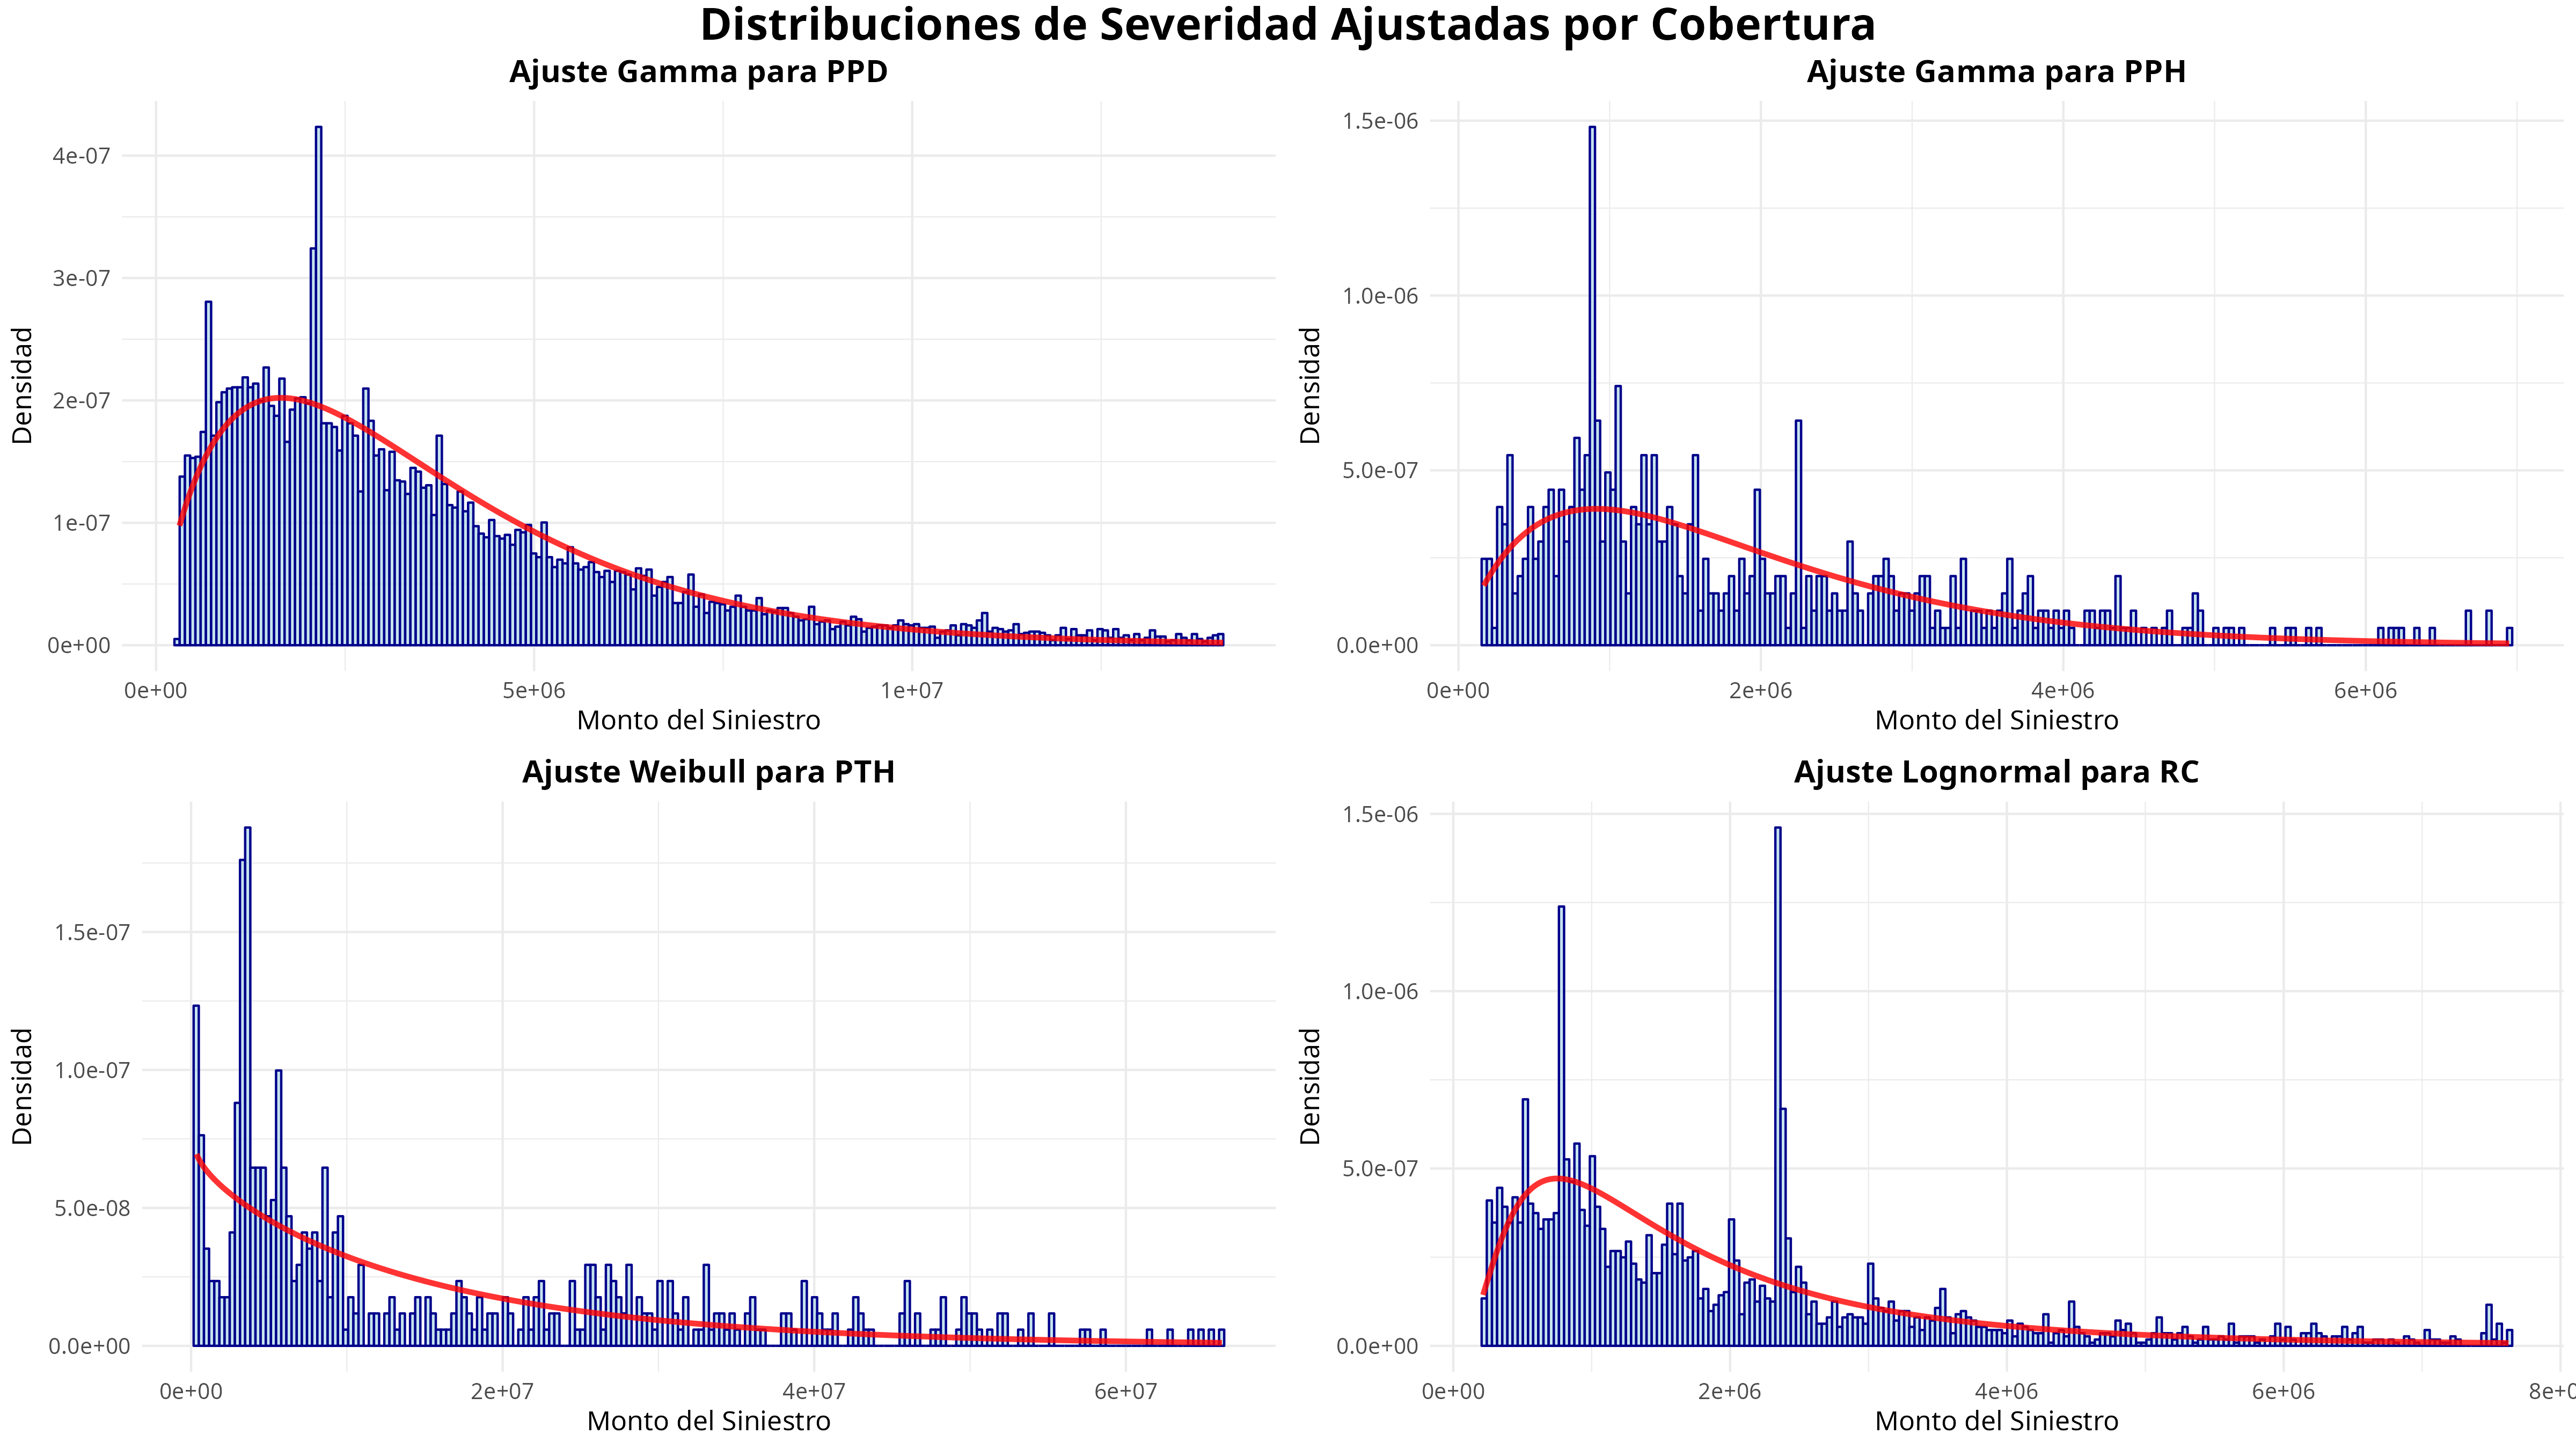
\includegraphics[width=0.8\textwidth]{../images/ajuste_distribuciones_severidad.png}
\caption{Ajuste de distribuciones teóricas sobre datos de severidad limpios por cobertura}
\end{figure}

\subsection{Algoritmo recursivo de Panjer}

La implementación del algoritmo de Panjer se desarrolló en la función \texttt{Panjer.R}, diseñada como wrapper de la librería \texttt{actuar} de R para modelos de suma aleatoria. El algoritmo utiliza el método recursivo \texttt{aggregateDist()} con configuración optimizada para manejar distribuciones discretizadas de gran dimensión y garantizar convergencia numérica estable.\\

El proceso incluye validación robusta de entrada que verifica la suma unitaria de probabilidades de severidad y implementa corrección automática mediante redistribución de masa en casos de concentración anómala. La función maneja múltiples distribuciones de frecuencia (Poisson, Binomial Negativa, Binomial y Geométrica) con conversión automática de parámetros según la especificación requerida por el algoritmo recursivo.

\begin{table}[H]
\centering
\caption{Configuración del algoritmo de Panjer por cobertura}
\begin{tabular}{lcccc}
\hline
\textbf{Cobertura} & \textbf{Distribución} & \textbf{Parámetros} & \textbf{P(S=0)} & \textbf{Convergencia} \\
\hline
PPD & Binomial Negativa & size=497.83, $\mu$=2.72 & 0.0665 & $<$50,000 iter. \\
PPH & Poisson & $\lambda$=0.114 & 0.8922 & $<$50,000 iter. \\
PTH & Binomial Negativa & size=70.56, $\mu$=0.104 & 0.9012 & $<$50,000 iter. \\
RC & Binomial Negativa & size=253.88, $\mu$=0.535 & 0.5858 & $<$50,000 iter. \\
\hline
\end{tabular}
\end{table}

La configuración técnica emplea 50,000 iteraciones máximas con tolerancia de convergencia de $1 \times 10^{-12}$ para garantizar precisión numérica. El algoritmo genera distribuciones de pérdida agregada con 50,001 puntos, proporcionando tanto funciones de masa de probabilidad (PMF) como de distribución acumulada (CDF) para análisis posterior.

\subsection{Transformada Rápida de Fourier}

La implementación del algoritmo FFT se desarrolló en la función \texttt{FFT\_RiesgoColectivo.R}, diseñada para calcular distribuciones de pérdida agregada mediante suma aleatoria utilizando propiedades de convolución en el dominio de frecuencia. Este método aprovecha la eficiencia computacional de la FFT para procesar vectores de gran dimensión con complejidad $O(n \log n)$ en lugar de $O(n^2)$ del método recursivo tradicional.\\

El algoritmo implementa padding automático a potencias de 2 (262,144 puntos) para optimizar la performance de la FFT y aplica truncamiento inteligente de la distribución de frecuencia basado en criterios de convergencia de masa de probabilidad. La función incluye validación robusta de normalización y manejo de valores negativos resultantes de errores de precisión numérica.

\begin{table}[H]
\centering
\caption{Configuración técnica del algoritmo FFT}
\begin{tabular}{lcccc}
\hline
\textbf{Cobertura} & \textbf{Puntos FFT} & \textbf{Truncamiento} & \textbf{Masa conservada} & \textbf{Error máximo} \\
\hline
PPD & 262,144 & n=9 & 99.94\% & $<1 \times 10^{-4}$ \\
PPH & 262,144 & n=2 & 99.98\% & $<1 \times 10^{-4}$ \\
PTH & 262,144 & n=2 & 99.98\% & $<1 \times 10^{-4}$ \\
RC & 262,144 & n=4 & 99.98\% & $<1 \times 10^{-4}$ \\
\hline
\end{tabular}
\end{table}

El proceso utiliza la fórmula de suma aleatoria $P(S = s) = \sum_{n=0}^{\infty} P(N = n) \cdot P(X_1 + \cdots + X_n = s)$, donde la convolución n-fold se calcula eficientemente mediante $\text{FFT}^{-1}[\text{FFT}(f_X)^n]$. La implementación incluye normalización automática y corrección de no-negatividad para garantizar la validez probabilística del resultado.

\subsection{Validación cruzada FFT vs Panjer}

La validación cruzada entre ambos algoritmos se implementó mediante análisis comparativo de las distribuciones resultantes, evaluando diferencias en funciones de masa de probabilidad (PMF) y funciones de distribución acumulada (CDF). El proceso incluye cálculo de métricas de error absoluto máximo y coeficientes de correlación para cuantificar la consistencia entre metodologías.

\begin{table}[H]
\centering
\caption{Métricas de validación cruzada FFT vs Panjer}
\begin{tabular}{lcccc}
\hline
\textbf{Cobertura} & \textbf{Error máx. PMF} & \textbf{Error máx. CDF} & \textbf{Corr. PMF} & \textbf{Corr. CDF} \\
\hline
PPD & $2.03 \times 10^{-4}$ & $5.03 \times 10^{-4}$ & $>0.9999$ & $>0.9999$ \\
PPH & $3.68 \times 10^{-5}$ & $1.68 \times 10^{-4}$ & $>0.9999$ & $>0.9999$ \\
PTH & $1.47 \times 10^{-4}$ & $2.89 \times 10^{-4}$ & $>0.9999$ & $>0.9999$ \\
RC & $1.89 \times 10^{-4}$ & $3.12 \times 10^{-4}$ & $>0.9999$ & $>0.9999$ \\
\hline
\end{tabular}
\end{table}

\begin{minipage}[T][4cm]{0.42\textwidth}
Los resultados confirman la equivalencia numérica entre ambos métodos, con errores máximos del orden de $10^{-4}$ y correlaciones superiores a 0.9999. Esta validación garantiza la robustez de las implementaciones y proporciona confianza en la selección del método FFT para el cálculo de la distribución agregada total debido a su superior eficiencia computacional.
\end{minipage}
\hfill
\begin{minipage}[B]{0.53\textwidth}
\centering
\includegraphics[width=\textwidth]{../data/output/grafico_validacion_cdf_fft_panjer.png}
\captionof{figure}{Validación cruzada: comparación de funciones de distribución acumulada FFT vs Panjer}
\end{minipage}

\subsection{Convolución final y distribución agregada total}

La implementación de la convolución final utiliza la función \texttt{convolucion\_fft()} personalizada para combinar las cuatro distribuciones de pérdida agregada individuales en una distribución total del portafolio. El proceso emplea convolución secuencial con padding automático a potencias de 2 para optimizar la performance computacional.\\

La metodología implementa escalamiento progresivo del dominio de cálculo: iniciando con 50,001 puntos para PPD, expandiendo a 100,001 tras convolución con PPH, 150,001 con PTH y finalmente 200,001 puntos tras inclusión de RC. Esta estrategia permite manejo eficiente de memoria mientras preserva resolución numérica.

\begin{table}[H]
\centering
\caption{Percentiles de la distribución agregada total del portafolio}
\begin{tabular}{lc}
\hline
\textbf{Percentil} & \textbf{Valor (millones COP)} \\
\hline
90\% & 24.58 \\
95\% & 30.85 \\
99\% (VaR) & 52.42 \\
99.9\% & 92.56 \\
\hline
\end{tabular}
\end{table}

El resultado final comprende una distribución de pérdida agregada total con rango de \$0 a \$2,000 millones COP, resolución de \$10,000 y validación completa de normalización probabilística. La implementación genera visualizaciones en doble escala (50M para análisis detallado, 500M para análisis de colas) y archivos de salida compatibles con análisis de riesgo posteriores.

\begin{figure}[H]
\centering
\includegraphics[width=1.0\textwidth]{../data/output/grafico_combinado_50M.png}
\caption{Distribución agregada total del portafolio (escala detallada hasta 50M COP)}
\end{figure}